\documentclass[12pt,onecolumn,a4paper]{article}
\usepackage{epsfig,graphicx,subfigure,amsthm,amsmath}
\usepackage{color,xcolor}     
\usepackage{xepersian}
\usepackage{cite}
\usepackage{fontspec}
\usepackage{multirow}

\settextfont[Scale=1]{BMitra}
\setlatintextfont[Scale=0.8]{Vazir-Regular}


\begin{document}
\title{گزارش تکلیف ۳ درس یادگیری ماشین} 
\author{کسرا سینایی\\
شماره دانشجویی ۸۱۰۶۹۶۲۵۴\\
}
\date{\today}
\maketitle
\thispagestyle{empty}
\newpage

\section{تمارین آماری}

\subsection{سوال یک}
\begin{figure}[h!]
    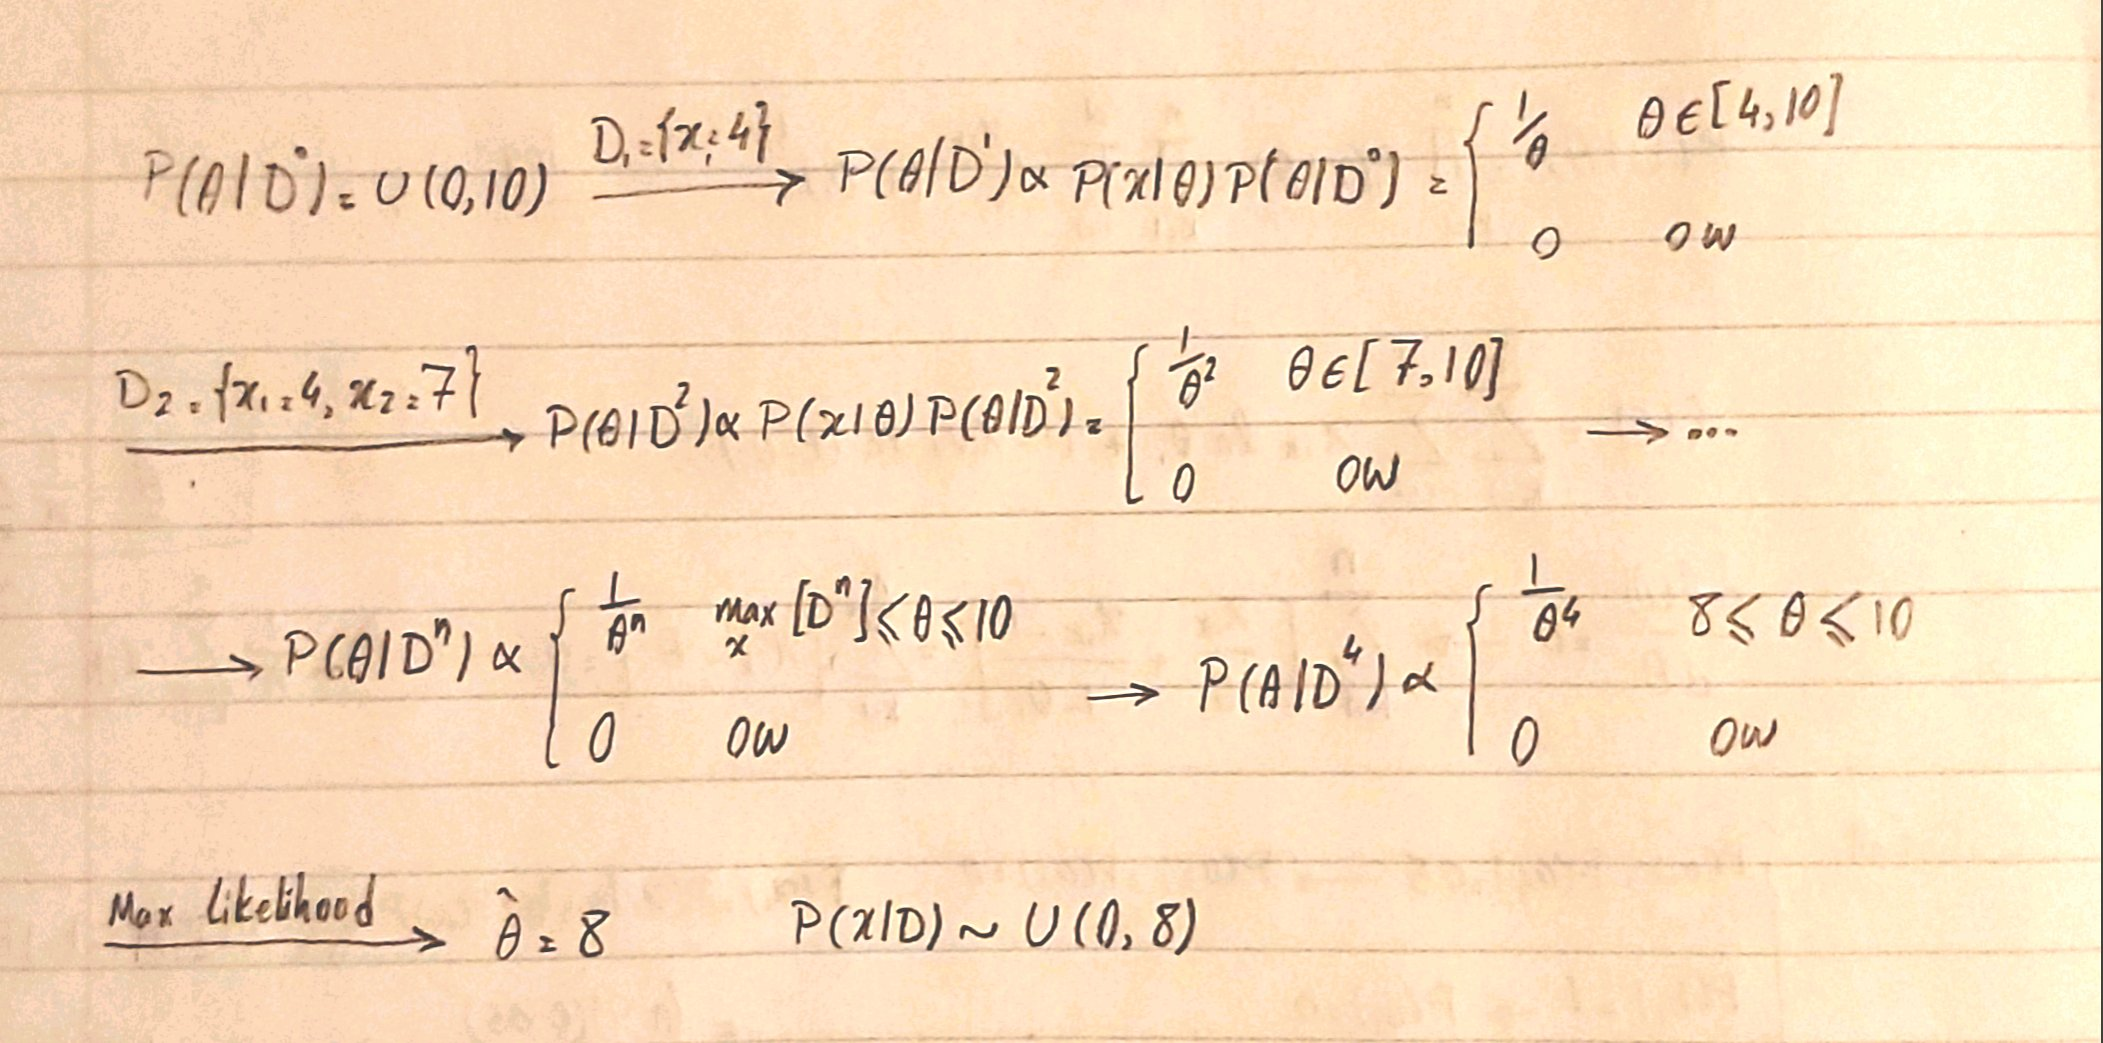
\includegraphics[width=\linewidth]{q1.jpg}    
\end{figure}

\subsection{سوال دو}
\begin{figure}[h!]
    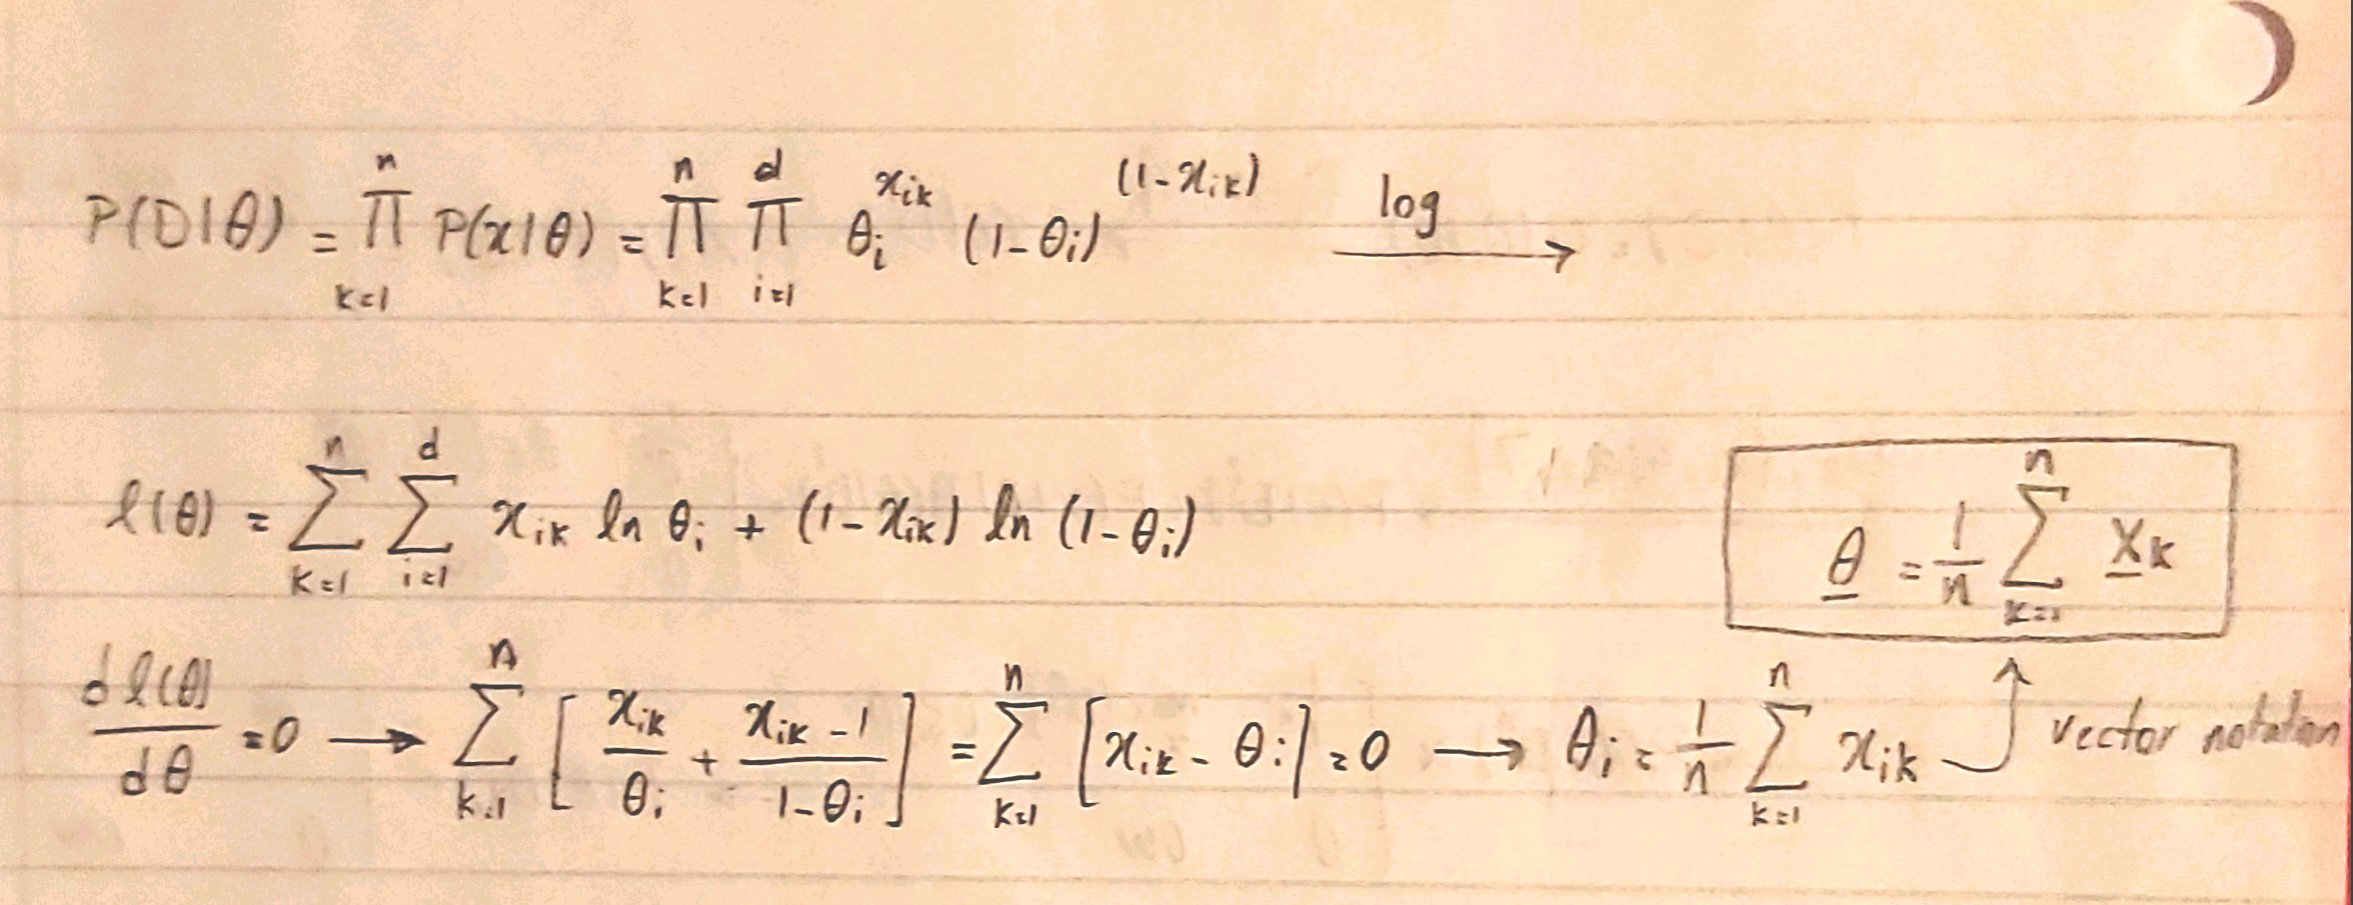
\includegraphics[width=\linewidth]{q2.jpg}    
\end{figure}
\newpage
\subsection{سوال چهار}
\begin{figure}[h!]
    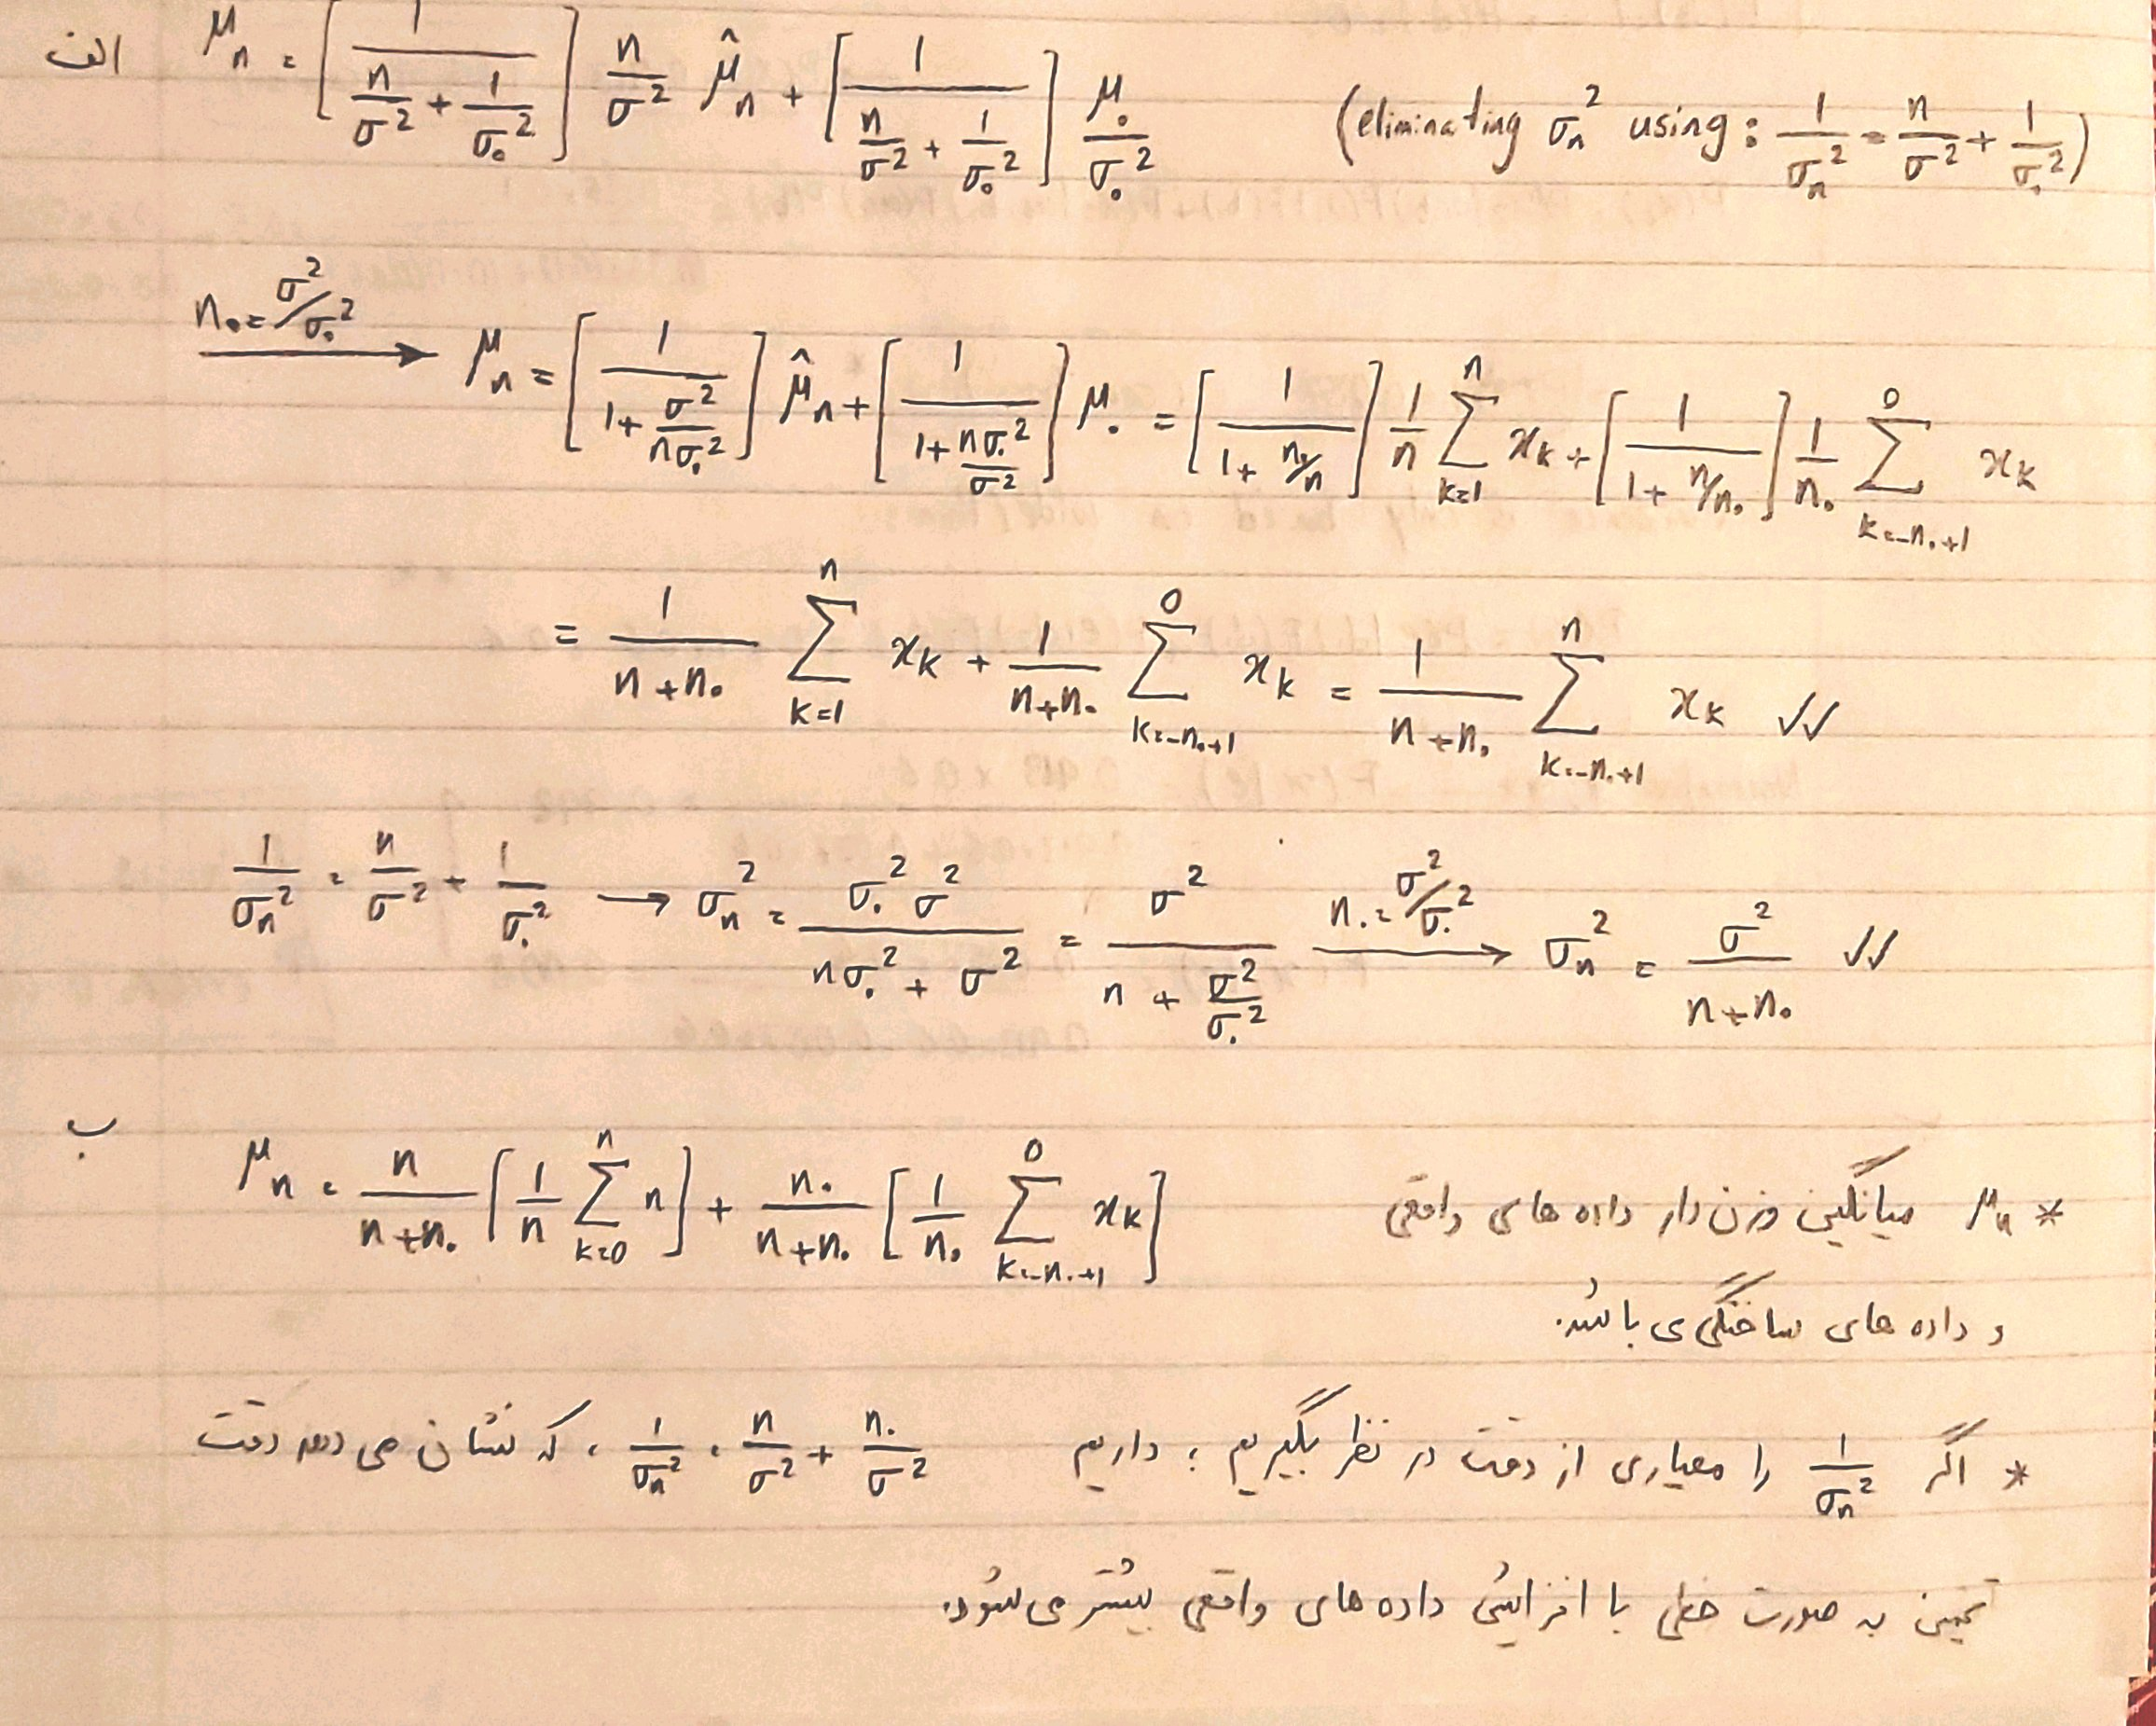
\includegraphics[width=\linewidth]{q4.jpg}    
\end{figure}
\newpage
\subsection{سوال هفت}
\begin{figure}[h!]
    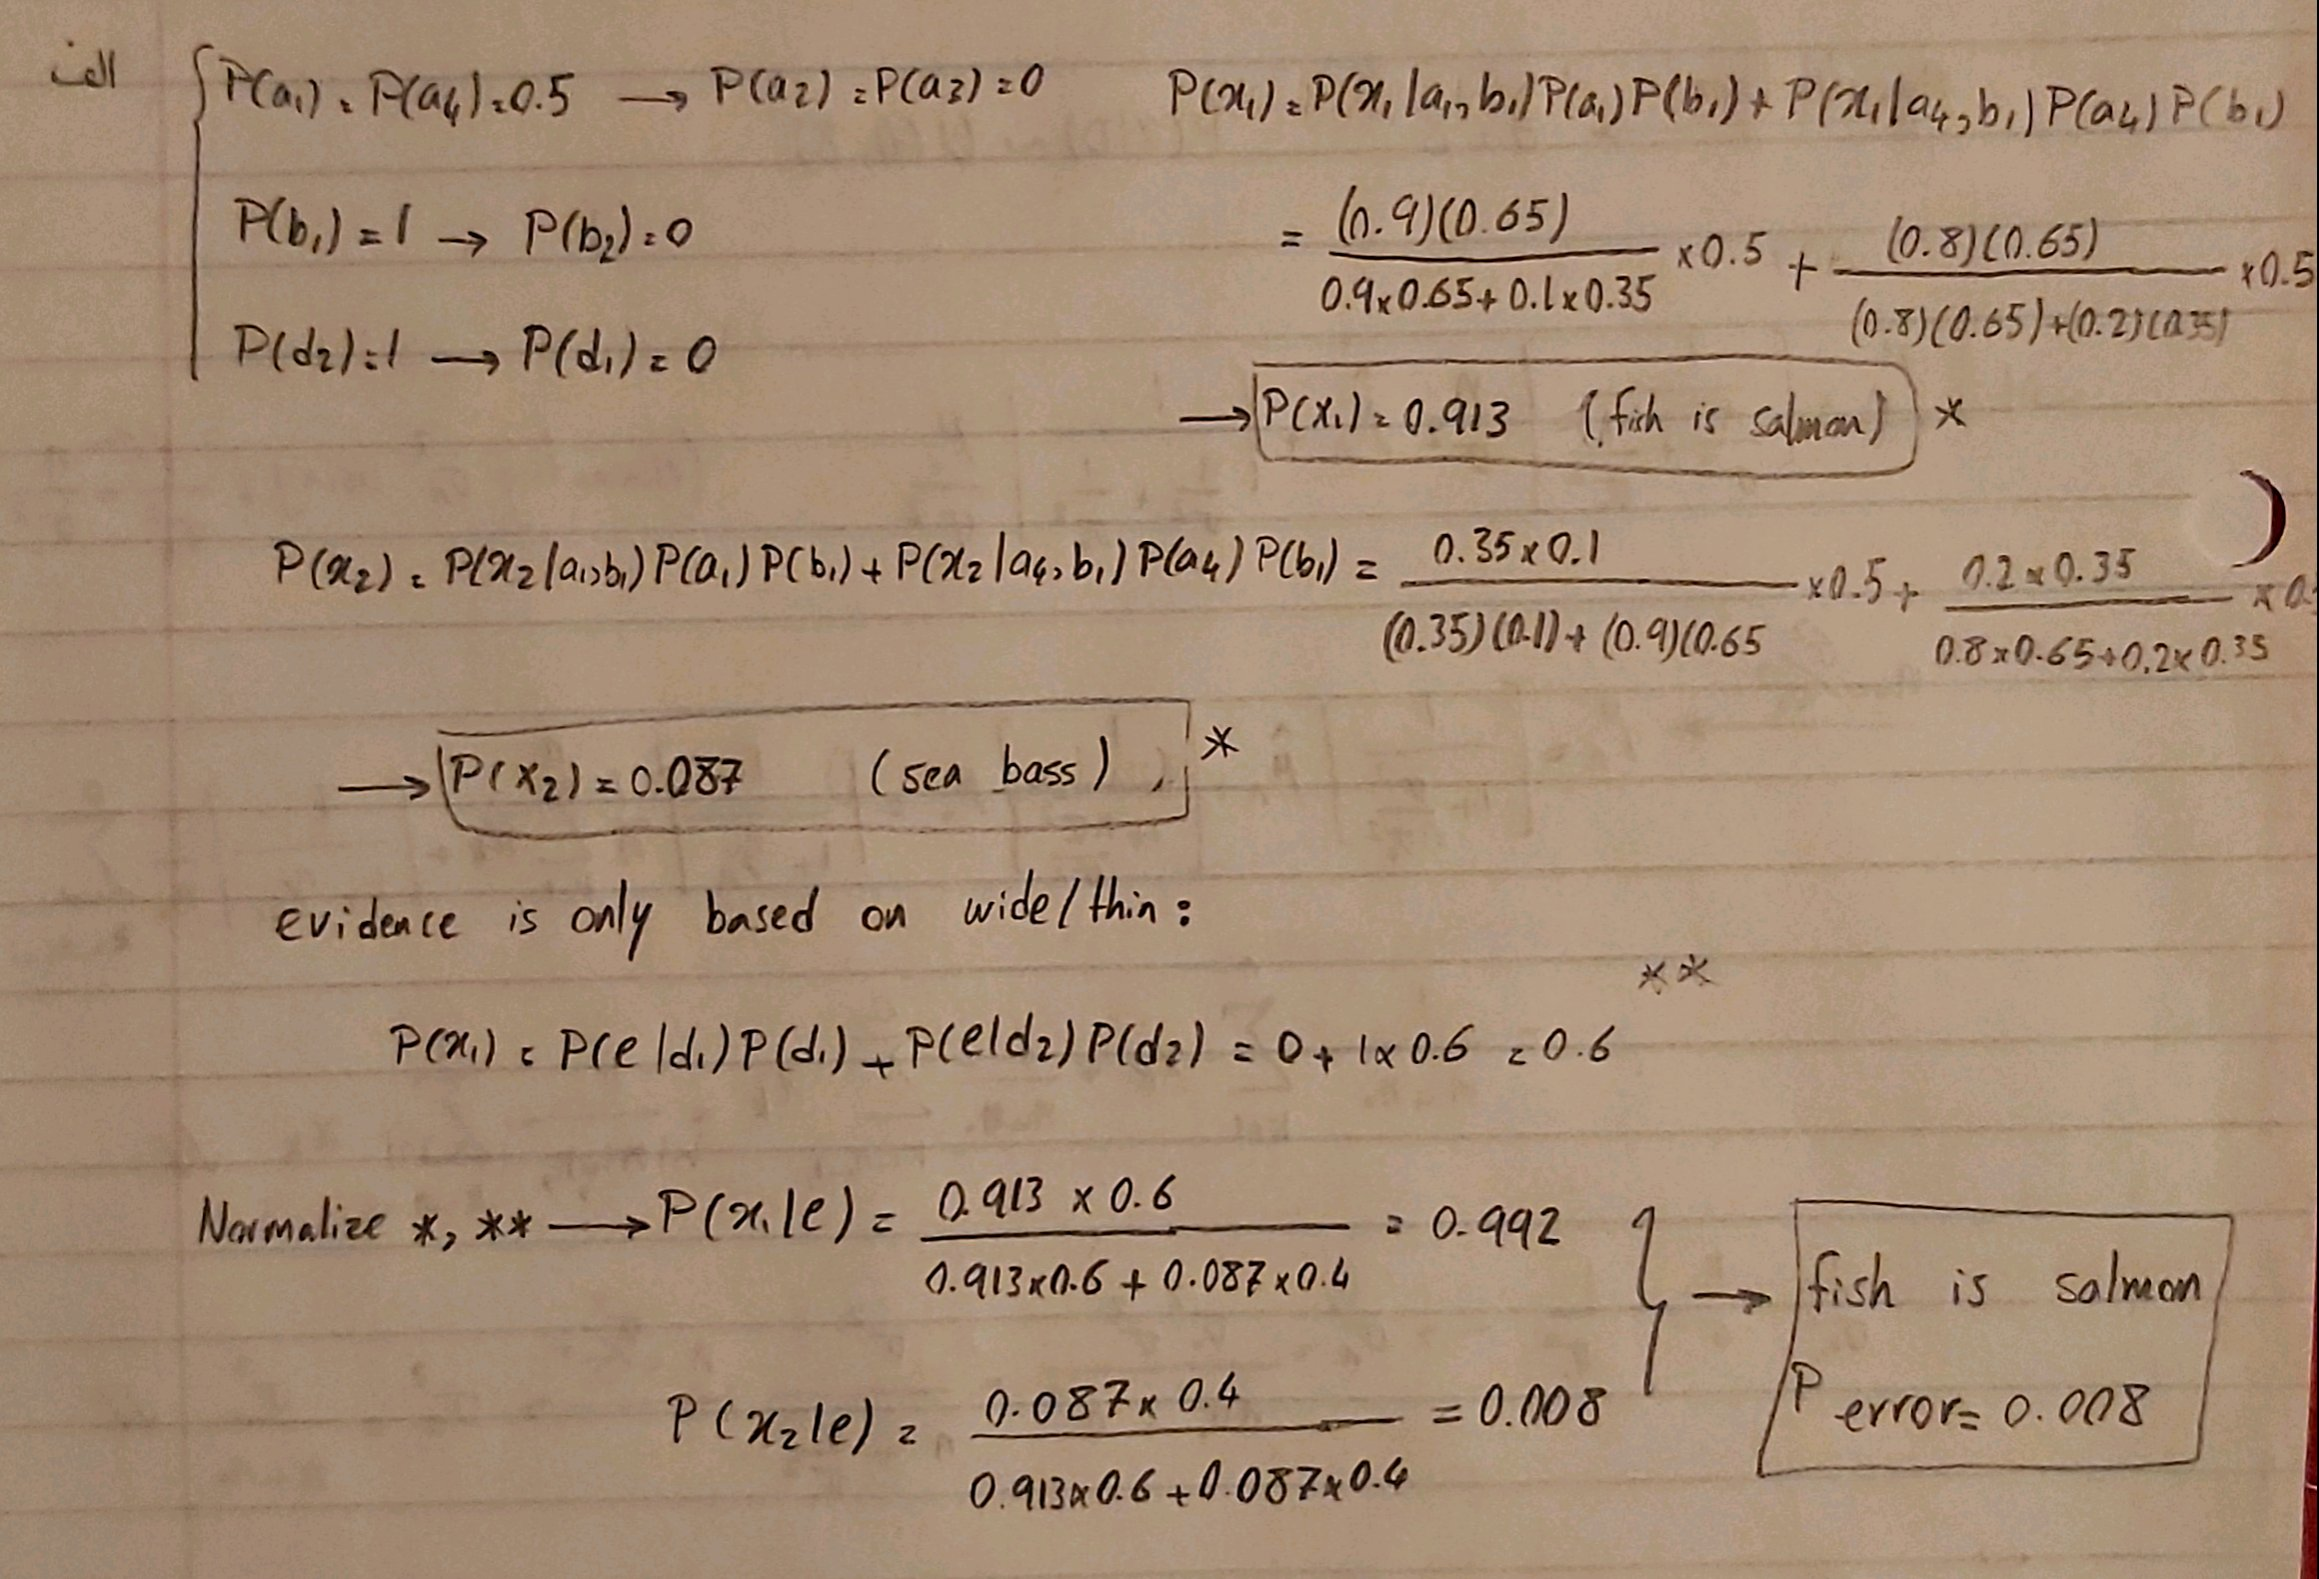
\includegraphics[width=\linewidth]{q7a.jpg}    
\end{figure}
\newpage
\begin{figure}[h!]
    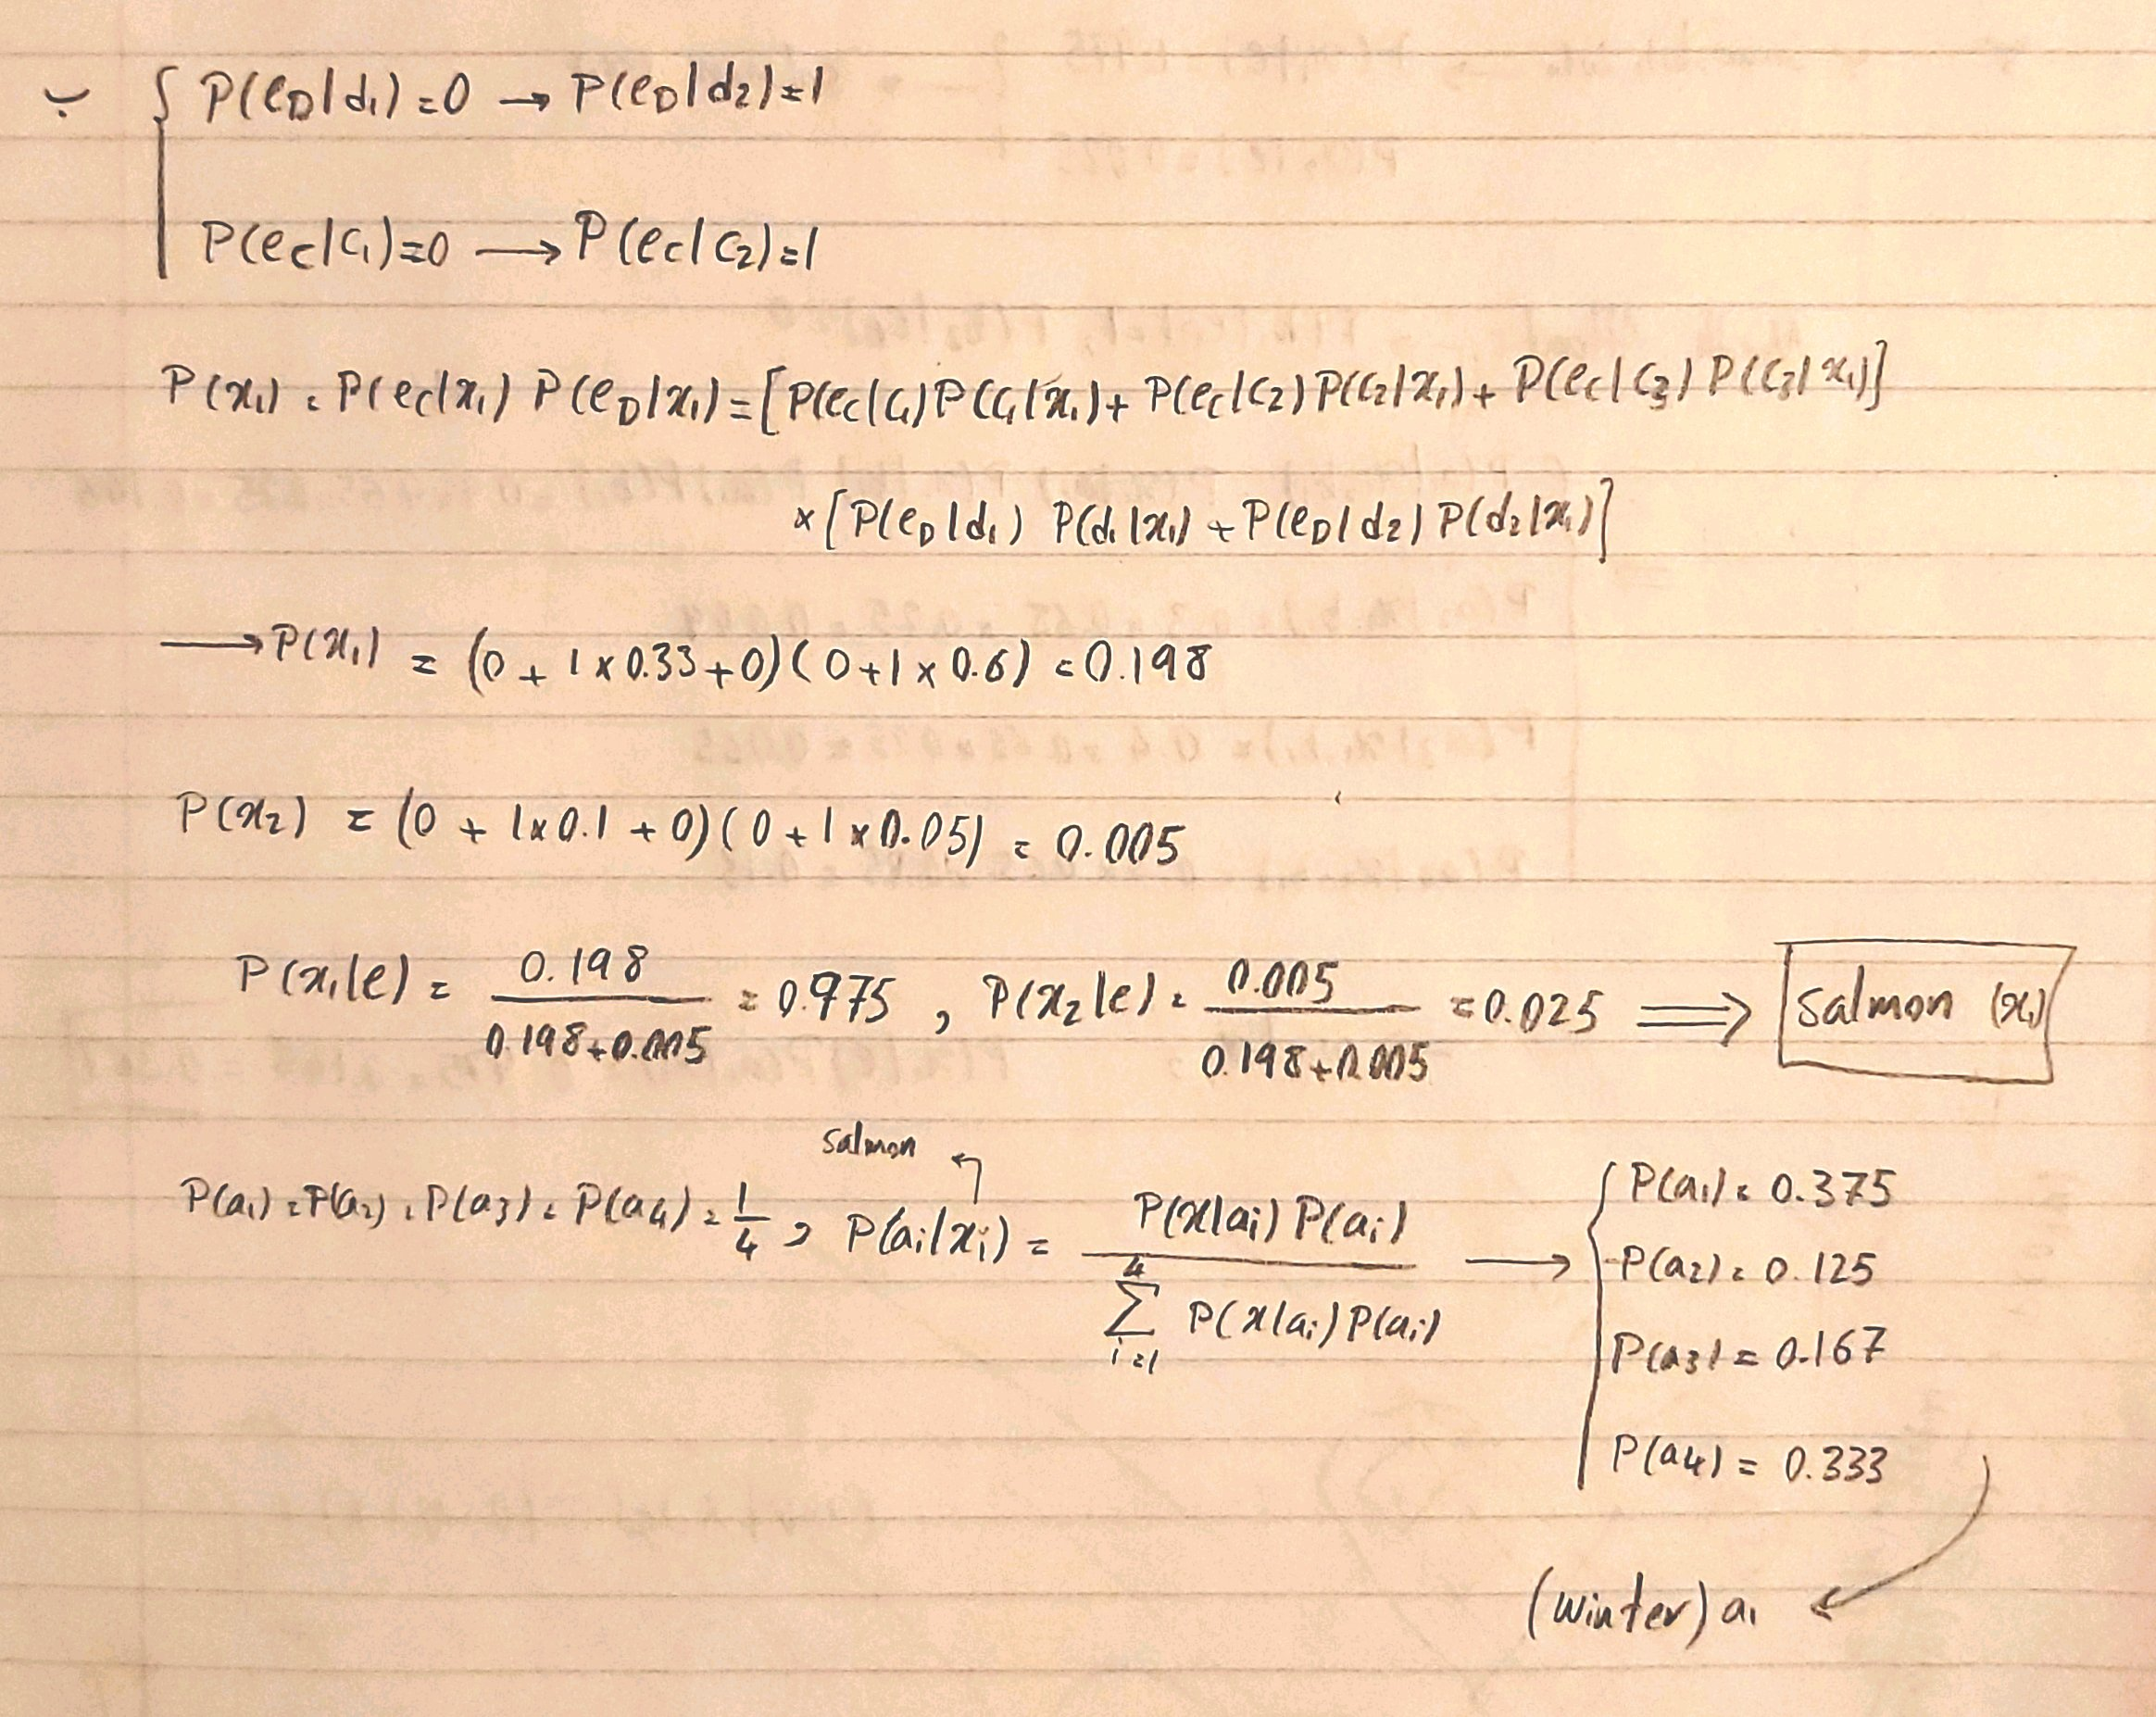
\includegraphics[width=\linewidth]{q7b.jpg}    
\end{figure}
\begin{figure}[h!]
    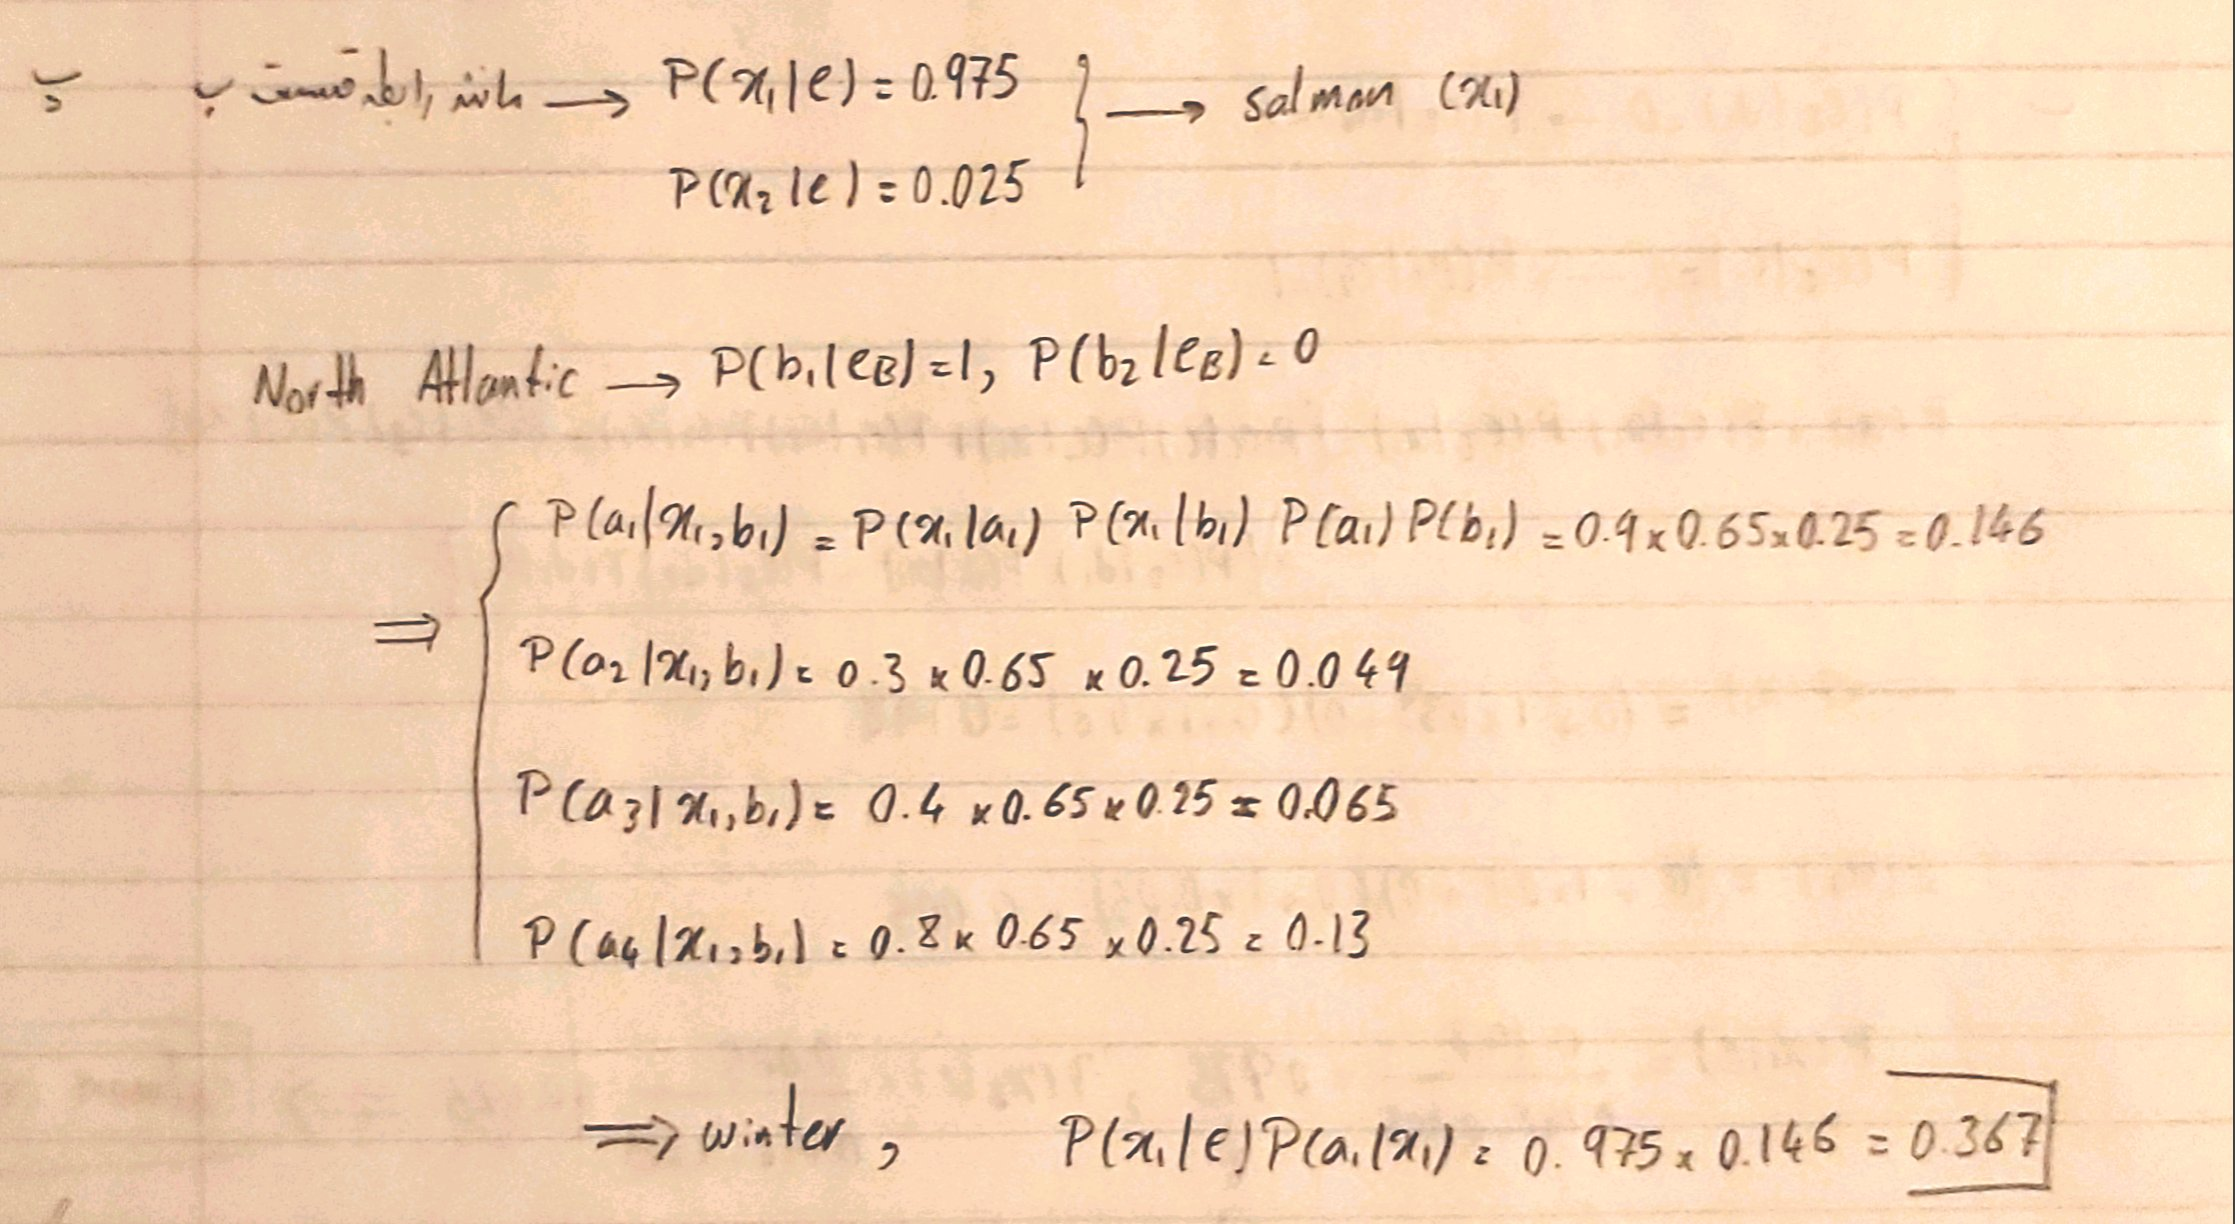
\includegraphics[width=\linewidth]{q7c.jpg}    
\end{figure}

\section{تمارین شبیه سازی}
\subsection{سوال هشت}
در این تمرین ابتدا با استفاده از کتابخانه \lr{OpenCV} عکس‌های موجود در پوشه مربوط به این سوال را لود کرده و تنها مقادیر مربوط به میانگین کانال \lr{R} و \lr{B} را به عنوان فیچر استخراج شده و به همراه لیلبل‌ها باز گردانده می‌شوند. تابع مورد استفاده در این سوال مشابه تمرین یک بوده و در فایل \lr{load pics py} پیاده سازی شده است.
\\
برای پیاده سازی طبقه بند در هر سه سوال  این تکلیف یک کلاس به نام \lr{GMM} پیاده سازی شده است که سه متد برای فیت کردن مدل و پیش‌بینی دارد:
\begin{description}
    \item[$\bullet$] \lr{constructor}: ابعاد فیچرها، تعداد کلاس‌ها و تعداد المان‌های میکسچر مدل را از کاربر می‌گیرد و یک لیست آبجکت \lr{mixture GaussianMixture} (از کتابخانه \lr{scikit learn}) با تعداد میکسچر تنظیم شده در آرگومان ورودی می‌سازد.
    \item[$\bullet$] \lr{update}: داده‌ها و لیبل‌ها را گرفته و برای هر کلاس پارامترهای میکسچر مدل را آپدیت می‌کند. (با استفاده از متد \lr{fit})
    \item[$\bullet$]  \lr{predict}: این تابع یک بردار با اندازه دلخواه از فیچرها می‌گیرد و با توجه به میکسچر مدل‌های یادگرفته شده لیبل آن‌ها را پیش‌بینی می‌کند. مبنای تصمیم گیری در این طبقه بند \lr{loglikelihood} میکسچر مدل‌ها برای هر یک از کلاس‌ها است. با استفاده از متد \lr{score samples} این مقدار به دست می‌آید.
\end{description}
تابع \lr{update} حاصل جمع مقادیر \lr{AIC} و \lr{BIC} را بازمی‌گرداند. میانگین‌ها و ماتریس کواریانس همه کلاس‌ها نیز پابلیک می‌باشد و می‌توان خراج از کلاس به آن‌ها دسترسی داشت و از آن‌ها برای ترسیم کانتورهای میکسچرمدل‌های کلاس‌ها استفاده کرد.
\\
تابع \lr{plot} برای ترسیم این کانتورها در هر سه سوال شبیه سازی این تکلیف استفاده شده‌است. این تابع چهار آرایه \lr{numpy} در آرگومان‌های ورودی خود دریافت می‌کند. آرایه اول در هر سطر خود میانگین یک توزیع گوسی را دارد، آرایه دوم ماتریس کواریانس متناظر با میانگین‌ توزیع‌های آرایه اول است، آرایه سوم و چهارم داده‌های سوال هستند که به صورت نقاط رنگی اسکتر می‌شوند. برای رسم کانتور نیز یک مش گرید در راستای \lr{x} و \lr{y} تشکیل می‌دهیم و با استفاده از تابع \lr{Multivariate Normal} از کتابخانه \lr{scipy} احتمال آن را حساب می‌کنیم و برای هر توزیع نرمال دو خط کانتور رسم می‌کنیم.
\\
نمودارهای \lr{AIC} و \lr{BIC} را پس از فیت کردن میکسچر مدل‌هایی با تعداد مدل ۲-۹ رسم می‌کنیم تا بر اساس آن بهینه ترین مدل برای این سوال را بیابیم.

\begin{figure}[t!]
    \label{fig:1}
    \begin{center}
    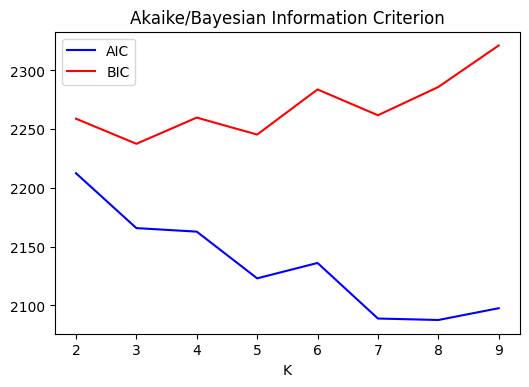
\includegraphics[scale=0.7]{q8_aicbic.png}
    \caption{نمودارهای \lr{Akaike/Bayes Information Criterion} به ازای مقادیر مختلف \lr{k}}
    \end{center}
\end{figure}
\newpage

با توجه به نمودار می‌توان نتیجه گرفت مقدار ۳ و ۷ برای مدل مناسب به نظر می‌رسند. حال کانتورهای مربوط به میکسچر مدل را برای این طبقه بند رسم می‌کنیم.

\begin{figure}[h!]
    \label{fig:2}
    \begin{center}
    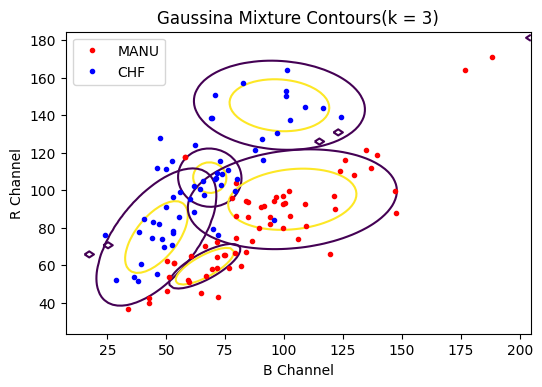
\includegraphics[scale=0.7]{q8_scatter.png}
    \caption{کانتور توزیع‌های گوسی مربوط به میکسچر مدل‌های دو کلاس}
    \end{center}
\end{figure}

برای این حالت پارامترهای مدل‌های گوسی فیت شده برای هر کلاس در جدول زیر گزارش شده‌اند. همچنین طبقه‌بند با تعداد مؤلفه‌های بالاتر (۴ و ۶) نیز آپدیت شد و کانتور مد‌های گاوسی آن پس از یادگیری در شکل زیر نشان داده شده‌اند. با توجه به نمدار \lr{BIC} تعداد مؤلفه بهینه برای این مسئله ۳ انتخاب شدُ تاثیر افزایش مؤلفه‌ها بر روی شکل کانتور توزیع‌های گاوسی طبقه بند برای هر یک از کلاس‌ها در شکل دیده می‌شود. تطابق بیش از اندازه بر روی داده‌های نویزی (عکس‌هایی که هم رنگ آبی و هم رنگ قرمز در آن‌ها به یک مقدار دیده می‌شد) لزوماً به بهبود عملکرد طبقه بند نمی‌انجامد.

\begin{figure}[h]
    \centering
    \subfigure[\lr{k = 4}]{
    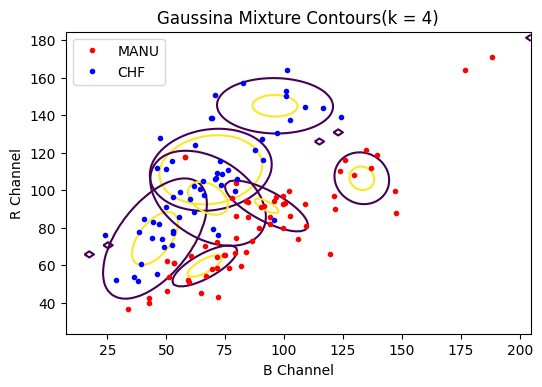
\includegraphics[width=.45\textwidth]{q8_4.png}
    }
    \subfigure[\lr{k = 6}]{
    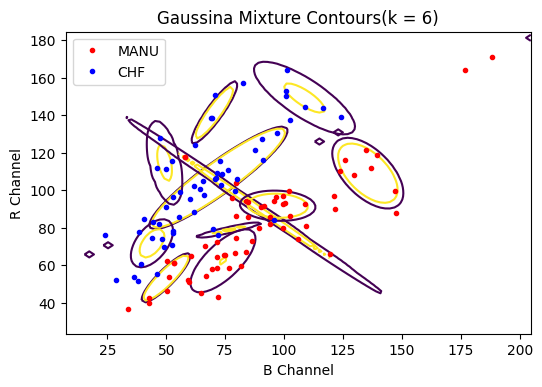
\includegraphics[width=.45\textwidth]{q8_6.png}
    }
    \caption{کانتورهای به دست آمده از طبقه‌بند با تعداد مؤلفه‌های بیشتر}
    \label{fig:8}
\end{figure}

\begin{center}
\begin{table}[h]
    \begin{centering}
        \begin{tabular}{|c|ccc|ccc|}
        \hline
            \multicolumn{1}{|c|}{\multirow{2}{*}{\lr{comp}}} & \multicolumn{3}{c|}{\lr{ManU}}    & \multicolumn{3}{c|}{\lr{CHF}}   \\ \cline{2-7} 
            \multicolumn{1}{|c|}{}   & \multicolumn{1}{c|}{\lr{weight}} & \multicolumn{1}{c|}{$\mu$} & $\sigma$ & \multicolumn{1}{c|}{\lr{weight}} & \multicolumn{1}{c|}{$\mu$}  & $\sigma$ \\ \hline
            \lr{1}      & \multicolumn{1}{c|}{\lr{0.46}}     & \multicolumn{1}{c|}{$\begin{pmatrix}68.4 & 106.6 \end{pmatrix}$} & $\begin{pmatrix} 169.1 & -4.9  \\  -4.9 & 226.12  \end{pmatrix}$    & \multicolumn{1}{c|}{\lr{0.03}}    & \multicolumn{1}{c|}{$\begin{pmatrix}182.4 & 167.4 \end{pmatrix}$} & $\begin{pmatrix} 33.6 & 20.7  \\  20.7 & 12.8  \end{pmatrix}$   \\ \hline
            \lr{2}      & \multicolumn{1}{c|}{\lr{0.34}}     & \multicolumn{1}{c|}{$\begin{pmatrix}45.8 & 74.9 \end{pmatrix}$} & $\begin{pmatrix} 99.9 & 87.3  \\  87.3 & 207.4  \end{pmatrix}$    & \multicolumn{1}{c|}{\lr{0.44}}    & \multicolumn{1}{c|}{$\begin{pmatrix}66.3 & 59.4 \end{pmatrix}$} & $\begin{pmatrix} 232.9 & 138.5  \\  138.5 & 144.8  \end{pmatrix}$   \\ \hline
            \lr{3}      & \multicolumn{1}{c|}{\lr{0.19}}     & \multicolumn{1}{c|}{$\begin{pmatrix}98.0 & 145.2 \end{pmatrix}$} & $\begin{pmatrix} 250.2 & -15.8  \\  -15.8 & 107.1  \end{pmatrix}$    & \multicolumn{1}{c|}{\lr{0.53}}    & \multicolumn{1}{c|}{$\begin{pmatrix}103.5 & 95.1 \end{pmatrix}$} & $\begin{pmatrix} 536.8 & 54.6  \\  54.6 & 193.0  \end{pmatrix}$   \\ \hline
        \end{tabular}
    \end{centering}
    \caption{پارامترهای مدل فیت شده}
\end{table}
\end{center}

\newpage
\subsection{سوال نه}
در این سوال ابتدا داده‌های سه کلاس را بر حسب فیچرهای خواسته شده دو به دو در نمودار به تصویر می‌کشیم تا تشخیص بدهیم کدام فیچرها برای طبقه‌بندی مناسب‌تر می‌باشند.

\begin{figure}[h!]
    \label{fig:3}
    \begin{center}
    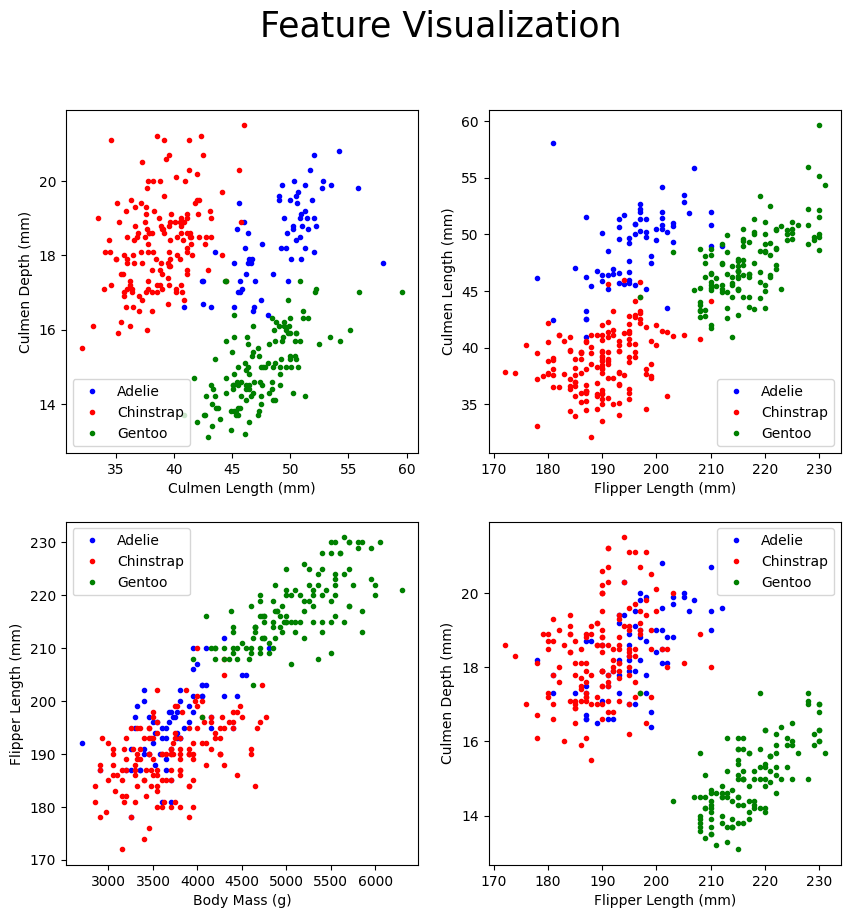
\includegraphics[scale=0.6]{q9_feature_comp.png}
    \caption{نمونه‌های مورد استفاده برای طبقه بندی پنگوئن‌ها}
    \end{center}
\end{figure}

تفکیک‌پذیری داده‌ها بر حسب دو فیچر \lr{culmen length} و \lr{culmen depth} از سایر مجموعه فیچرهای خواسته شده در صورت سوال بهتر به نظر می‌رسند. داده‌های مربوط به سه گونه مختلف پنگوئن‌ بر حسب این دو ویژگی از یکدیگر بیشتر فاصله داشته و نمونه‌های استثنایی کمتر به چشم می‌خورند.
\\
در قسمت بعدی تمرین با استفاده از کلاس \lr{GMM} که در سوال ۸ همین تمرین نیز از آن استفاده شد، طبقه بندهایی بر مبنای میکسچر مدل‌های گوسی با تعداد مؤلفه‌های مختلف فیت می‌کنیم. بر حسب دقت طبقه بند بر روی مجموعه داده‌ی تست مشخص می‌کنیم که کدام مجموعه فیچر برای طبقه بندی بهتر می‌باشد. دقت حالات مختلف طبقه‌بندی در جدول زیر آورده شده‌اند.
\begin{center}
\begin{table}[h!]
    \begin{tabular}{|c|c|c|}
        \hline
        \lr{Accuracy} & \lr{Feature Set} & \lr{GMM Components}     \\ \hline
        \lr{98.5}  & 1           & \multirow{4}{*}{2} \\ \cline{1-2}
        \lr{95.6}  & 2           &                    \\ \cline{1-2}
        \lr{79.7}  & 3           &                    \\ \cline{1-2}
        \lr{78.2}  & 4           &                    \\ \hline
        \lr{97.1}  & 1           & \multirow{4}{*}{3} \\ \cline{1-2}
        \lr{95.6}  & 2           &                    \\ \cline{1-2}
        \lr{81.1}  & 3           &                    \\ \cline{1-2}
        \lr{84.0}  & 4           &                    \\ \hline
        \lr{97.1}  & 1           & \multirow{4}{*}{4} \\ \cline{1-2}
        \lr{95.6}  & 2           &                    \\ \cline{1-2}
        \lr{81.1}  & 3           &                    \\ \cline{1-2}
        \lr{81.1}  & 4           &                    \\ \hline
        \lr{98.5}  & 1           & \multirow{4}{*}{5} \\ \cline{1-2}
        \lr{95.6}  & 2           &                    \\ \cline{1-2}
        \lr{81.1}  & 3           &                    \\ \cline{1-2}
        \lr{81.1}  & 4           &                    \\ \hline
    \end{tabular}
    \caption{دقت مدل‌های فیت بر روی مجموعه فیچرهای مختلف}
\end{table}
\end{center}
در داده‌های این سوال تعدادی از فیچرها در برخی از سمپل‌ها ناقص و نامعلوم بودند. با توجه به اینکه تعداد این موارد در کل دیتاست درصد قابل اغماضی بود با استفاده از \lr{imputer} میانه، فیچرهای نامعلوم جاگذاری شدند. انتظار می‌رود تغییر چندانی در عملکرد نهایی طبقه بند مشاهده نشود، چون تعداد این موارد جمعاً به ده نمی‌رسید.
\\
برای رسم کانتور توزیعذهای فیت شده با استفاده از زیرمجموعه‌های مختلف از دیتاست تعداد مؤلفه‌ها را برابر با ۲ در کلاس \lr{GMM} تنظیم می‌کنیم و با دیتا‌ست‌های مختلف مدل را آپدیت می‌کنیم. کانتورهای به دست آمده برای برای هر زیرمجموعه از دیتا ست و دقت طبقه‌بند بر روی مجموعه تست در تصاویر زیر نشان داده شده‌اند.

\begin{figure}[h]
    \centering
    \subfigure[فیچرهای ۱]{
    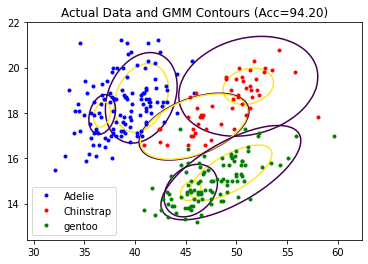
\includegraphics[width=.45\textwidth]{q9_1.png}
    }
    \subfigure[فیچرهای ۲]{
    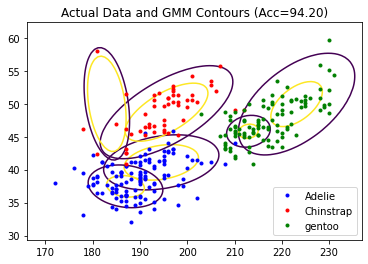
\includegraphics[width=.45\textwidth]{q9_2.png}
    }
    \subfigure[فیچرهای ۳]{
    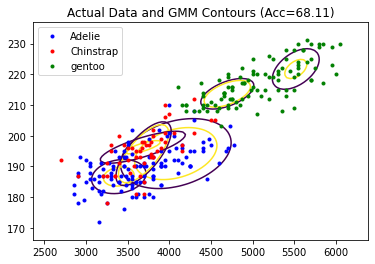
\includegraphics[width=.45\textwidth]{q9_3.png}
    }
    \subfigure[فیچرهای ۴]{
    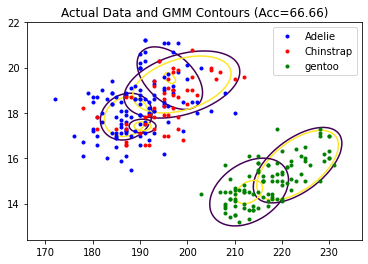
\includegraphics[width=.45\textwidth]{q9_4.png}
    }
    \caption{کانتور توزیع‌های گاوسی مربوط به میکسچرمدل با تعداد مؤلفه‌های متفاوت}
    \label{fig:6}
\end{figure}

\newpage
~\newpage
\subsection{سوال ده}
در این سوال عملکرد طبقه‌بند ساده بیزی را با عملکرد طبقه‌بندی با مدل \lr{GMM} مقایسه می‌کنیم.
\\
ابتدا همانند تکالیف قبلی با استفاده از الگوریتم \lr{optimal bayes} و بدون دانش اولیه \lr{(prior)} داده‌ها را طبقه‌بندی می‌کنیم. کانتور مدل‌های گاوسی به دست آمده برای تصمیم‌گیری بیز در شکل زیر نشان داده شده‌اند. دقت طبقه بند در این حالت برابر ۸۸ درصد می‌باشد.

\begin{figure}[h!]
    \label{fig:4}
    \begin{center}
    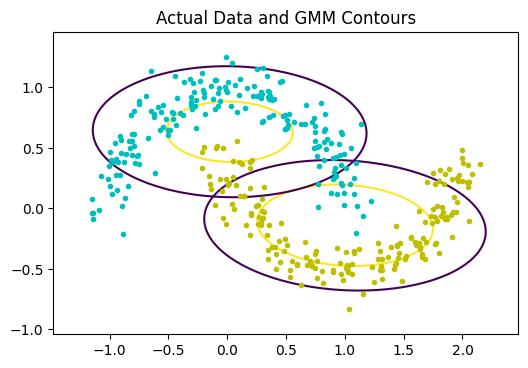
\includegraphics[scale=0.6]{q10_bayes.png}
    \caption{توزیع‌های به دست آمده توسط تخمین‌گر بیزی ساده}
    \end{center}
\end{figure}

برای آنکه بتوان از کلاس \lr{GMM} نوشته شده برای سؤالات قبلی استفاده کرد یک کلاس به نام \lr{GaussianMixture} همانند آبجکت موجود در کلاس سای‌کیت‌لرن پیاده سازی می‌کنیم. نام متغییرهای غیرخصوصی این کلاس مانند \lr{means}، \lr{covariances} و \lr{weights} می‌گذاریم. متدهای زیر برای اجرای الگوریتم \lr{EM} باید پیاده سازی شوند.
\begin{description}
    \item[$\bullet$] \lr{constructor}: آرایه‌های نام‌پای با طول متناسب با ابعاد فیچر و تعداد مؤلفه‌های میکسچر مدل برای میانگین، واریانس و وزن توزیع‌ها تشکیل می‌دهد.
    \item[$\bullet$] \lr{fit}: داده‌های ترین را به همراه تعداد ایتریشن می‌گیرد و به طور متوالی \lr{E Step} و \lr{M Step} را انجام می‌دهد.
    \item[$\bullet$] \lr{e step}: در این متد متغییر \lr{z} که همان \lr{latent variable} در الگوریتم \lr{EM} می‌باشد را با استفاده از تخمین کنونی پارامترهای میکسچر مدل به روز رسانی میذکنیم.
    \item[$\bullet$] \lr{m step}: در این متد پارامترهای مدل ($\mu_{i}$ُ، $\Sigma_{i}$ و $p_{i}$) را با استفاده از آخرین تخمین به دست آمده از متغییر دیده نشده محاسبه و به روزرسانی می‌کنیم.
    \item[$\bullet$] \lr{log likelihood}: لوگ‌لایکلیهود را برای داده‌های آرگومان ورودی بر حسب پارامترهای فعلی مدل محاسبه می‌کند. این تابع برای محاسبه \lr{AIC} و \lr{BIC} لازم می‌شود.
    \item[$\bullet$] \lr{aic}: مقدار \lr{AIC} را با استفاده از رابطه $$\operatorname{AIC}(G)=-2 \log \ell_{o}\left(\hat{\theta}_{G} ; G\right)+2 v_{G}$$ محاسبه می‌کند
    \item[$\bullet$] \lr{bic}: مقدار \lr{BIC} را با استفاده از رابطه $$\mathrm{BIC}(G)=-2 \log \ell_{o}\left(\hat{\theta}_{G} ; G\right)+v_{G} \log (n)$$ محاسبه می‌کند.
\end{description}
حال برای تشخیص دادن بهترین میکسچر مدل برای طبقه‌بند این سوال تعداد مؤلفه‌های مکیشچر مدل طبقه‌بند را از ۲ تا ۱۶ تغییر می‌دهیم و با رسم نمودار \lr{AIC} و \lr{BIC} بهینه‌ترین تعداد برای مؤلفه‌ها را می‌یابیم. این اطلاعات در شکل زیر نمایش داده شده‌اند.
\begin{figure}[h!]
    \label{fig:5}
    \begin{center}
    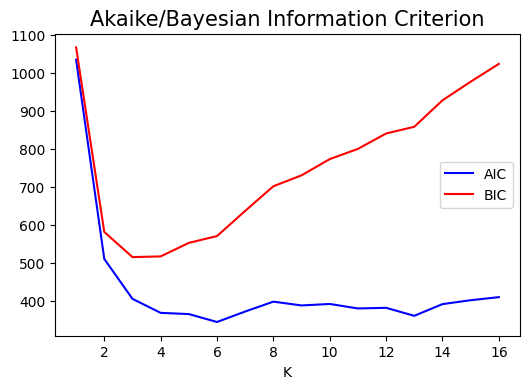
\includegraphics[scale=0.6]{q10_aicbic.png}
    \caption{تاثیر تعداد مؤلفه‌های میکسچرمدل گاوسی}
    \end{center}
\end{figure}

برای رسم نمودارها و طبقه‌بندی در این سوال نیز همان کلاس پیاده سازی شده در سوال ۸ استفاده شده است. 

\begin{figure}[h]
    \centering
    \subfigure[\lr{k = 3}]{
    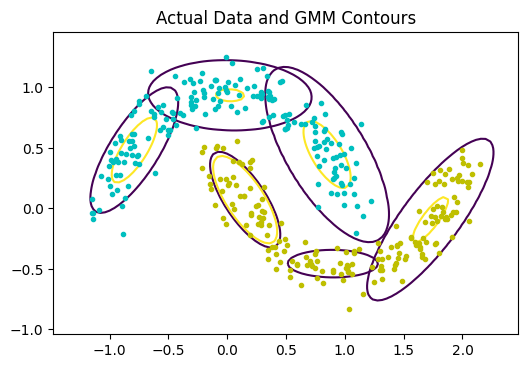
\includegraphics[width=.45\textwidth]{q10_3.png}
    }
    \subfigure[\lr{k = 8}]{
    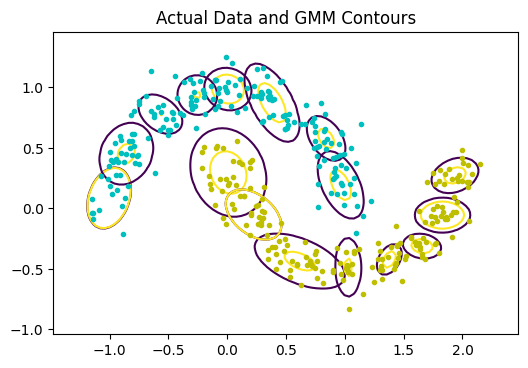
\includegraphics[width=.45\textwidth]{q10_8.png}
    }
    \subfigure[\lr{k = 16}]{
    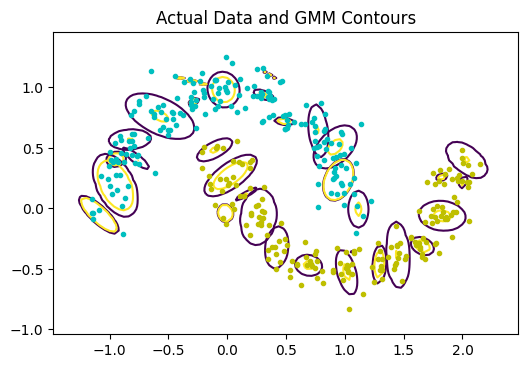
\includegraphics[width=.5\textwidth]{q10_16.png}
    }
    \caption{کانتور توزیع‌های گاوسی مربوط به میکسچرمدل با تعداد مؤلفه‌های متفاوت}
    \label{fig:7}
\end{figure}

\end{document}